\documentclass[14pt,a4paper]{extarticle}


\setlength{\topmargin}{-2cm}
\setlength{\oddsidemargin}{0cm}
\setlength{\textheight}{24cm}
\setlength{\textwidth}{16cm}



\usepackage{graphicx}
\usepackage{listings}
\usepackage[export]{adjustbox}
\usepackage{amsmath}
\usepackage{algorithm}
\usepackage[noend]{algpseudocode}

%Use helvetica as sans serif
\usepackage{helvet}



\begin{document}


\title{LINE FOLLOWING BEHAVIOR FOR AN AUTONOMOUS MOBILE ROBOT USING ARTIFICIAL NEURAL NETWORKS}

\author{Manash Kumar Mandal\\ 1203043 \\ Department of Electrical \& Electronic Engineering \\ Khulna University of Engineering \& Technology}

\date{}

\maketitle
	

\tableofcontents

\newpage


\begin{abstract}

In order to achieve tasks by the mobile robots, these robotic systems must have been intelligent and should decide their own action. To guarantee the autonomy and the intelligence for line following behavior, it is necessary to use the techniques of artificial intelligence like the artificial neural networks. This project report presents an approach for line following task by an autonomous mobile robot using a single layer neural network. The proposed controller is used for following any line on a plain surface with different width. This controller can also be upgraded to determine the value of $k_{p}$ and $k_{d}$ and make the autonomous line following a $PD$ controller based. The results acquired from Neural Network simulation and implementation on the robot are shown and discussed.

\end{abstract}

\providecommand{\keywords}[1]{\textbf{\textit{Keywords-}} #1}

\keywords{Feedforward Neural Network, Machine Learning, Robotics, Backpropagation Algorithm, Stochastic Gradient Descent, Proportional Derivative Controller}

\section{Introduction}

The line follower is a self operating robot that detects and follows a line that is drawn on the floor. The path consists of a black line on a white surface (or it may be reverse of that). The control system used must sense a line and maneuver the robot to stay on course, while constantly correcting the wrong moves using feedback mechanism, thus forming a simple yet effective closed loop system. The robot is designed to follow very tight curves. 

In this project, the conventional control system is being replaced by artificial neural network. 

	\subsection{Line detection mechanism}
	Line can be detected by either using Infra-red (IR) sensors, Light Dependent Resistor (LDR) or by a camera with line detection algorithms. Line tracking is a very important notion in the world of robotics as it give to the robot a precise, error-less and easy to implement navigation scheme. 
	
		\paragraph{Detecting line using IR}
		To detect line using IR, a threshold value must be measured. IR sensor gives different reading on different colored surface. Both values from IR on white line and IR on black line must be recorded before sensing the line.
		
		
		\begin{figure}[!h]
				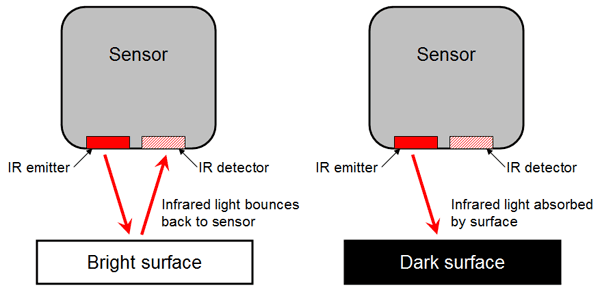
\includegraphics[width=\textwidth]{ir_line.png}
				\caption{Detecting line using IR sensor}
				\label{fig:detect_line_ir}
		\end{figure}
		
		\paragraph{Detecting line using LDR}
		To detect line using LDR same procedure from IR can be used. Since reflected line intensity depends on the reflecting surface. If the color of the surface is white, maximum light is reflected. If it is black then minimum light is reflected. Reflected light has different intensity based on the color of the surface it is being reflected from. So, nearest colors can be differentiated using LDR sensors. 
		
		\begin{figure}[!h]
			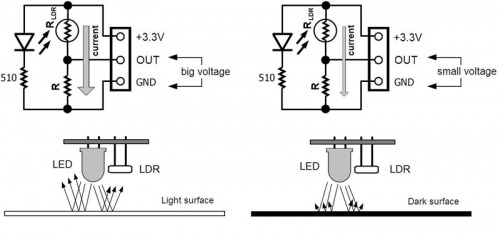
\includegraphics[width=\textwidth]{ldr_line.jpg}
			\caption{Detecting line using LDR sensor}
			\label{fig:detect_line_ldr}
		\end{figure}
		
		%Algorithm code
		
			\subsection{Algorithm for detecting line}
		\begin{algorithm}
		\caption{Line Detecting Algorithm}\label{alg:linetracker}
		\begin{algorithmic}[1]
		\Procedure{detectLine}{\textit{irPin}}
		
		\State $irPin \gets \text{ir receiver pin}$
		\State $irReading \gets \text {analog reading from ir receiver} $
		\State $threshold \gets \text {threshold value for differentiate betweeen white and black line} $
		\State $irDigitalReading \gets \text {converts analog into binary format} $
		
		\State $ irReading \gets \text{reading from irPin}$		
		\If {$irReading > \textit{threshold}$}
		\State $irDigitalReading \gets 1$
		\Else 
		\State $irDigitalReading \gets 0$
		\EndIf
		\EndProcedure
		\end{algorithmic}
		\end{algorithm}
	
	\subsection{Getting current position of the robot using IR / LDR Array}
	Current position of a robot on a line can be extracted by using IR array consisting of two or more than two IR/LDR sensors. Suppose, a robot has an IR array of 5 IR sensors. The spacing between two IR sensor is \textbf{1cm}, and the width of the line is \textbf{1.5cm}. At any time, when the robot is on the line, two values will differ from other three values meaning robot is facing straight, leaning left or leaning right. Depending on the position of the robot on the line, speed of motors can be varied to keep it on the line. This process is completely experimental and varies with the body, circuitry, battery rating, motor rating and mostly other things. The position value can be returned either in binary form such as \textbf{01100} using \ref{alg:linetracker} or in weighted value such as \textbf{2500} from \ref{alg:calculate_position}.
	
	
	\subsubsection{Algorithm for weighted positional value}
	\begin{algorithm}[H]
			\caption{Position calculating algorithm}\label{alg:calculate_position}
			\begin{algorithmic}[1]
			\Procedure{calculatePosition}{\textit{numberOfSensors}}
			\State $numberOfSensors	\gets \text{number of ir/ldr	sensors}$	
			\State  $numberOfActiveSensors \gets 0$
			\State  $digitalReading[numberOfSensors]$ be new array
			\State $weightedValues \gets 0$
			\State $weight \gets 1000$ \Comment{Setting weighted value 1000}
			\State  $position \gets -1$\Comment{Setting current position at -1}
			\For {$index \gets 0$ to $numberOfSensors$}
				\State $digitalReading[index] \gets \Call{detectLine}{index}$
				\If {$digitalReading[index] \gets 1$}
					\State $numberOfActiveSensors \gets numberOfActiveSensors + 1$
				\EndIf
				\State $weightedValues \gets weightedValues + digitalReading[index] * weight$
			\EndFor
			\State $position \gets weightedValues / numberOfActiveSensors$
			\State \textbf{return} $position$
			\EndProcedure		
	\end{algorithmic}
\end{algorithm}
	
	


	\subsection{Conventional line following mechanism}
	
	Conventional line following robots follow lines on a surface based on either predefined conditions or line patterns. Position of the robot can be calculated from  \ref{alg:calculate_position}. If the position of the sensor indicates the robot is being shifted to right from mid point of the line, then the speed of left motor is increased and right motor is decreased and vice versa. If the position of the robot is at middle point then both of the motor will go in the same direction with same speed. The procedure can be viewed from figure \ref{fig:differential_drive_image}.
	
		\begin{figure}[H]
			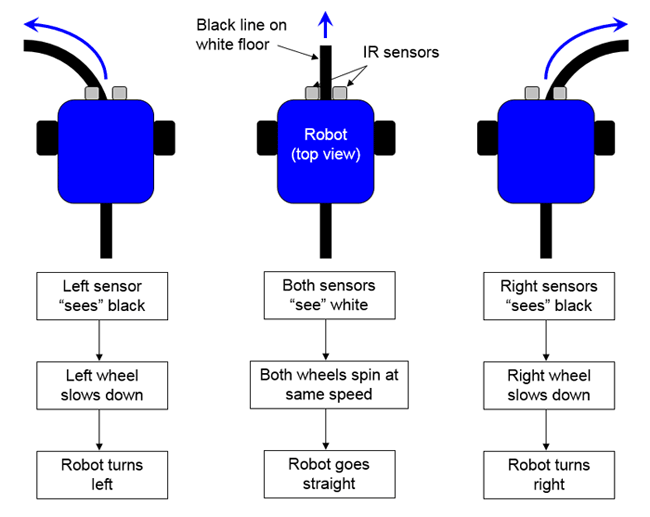
\includegraphics[width=\textwidth]{line-tracking-robot-steering.png}
			\caption{Differential steering drive for following line}
			\label{fig:differential_drive_image}
		\end{figure}
		
	
	\subsection{Drawbacks of line following robot based on differential drive system}
	
	Some drawbacks of differential drive system
	
		\begin{enumerate}
		\item It is a static method that can only be used on a specific robot for which the algorithm was designed
		\item Conditional statements varies with 
			\begin{enumerate}
				\item Weight of the robot
				\item Speed of the robot
				\item Spacing between the IR/LDR sensors of the sensor array
				\item Number of IR/LDR sensors used to make the array
				\item Width of the line to be followed by the robot
			\end{enumerate}
		
		\item This method is not appropriate for driving the robot in right and acute angle turns
		
		
		\end{enumerate}
		
	\section{Machine Learning}
	
	Machine learning is a subfield of computer science that evolved from the study of pattern recognition and computational learning theory in artificial intelligence. In 1959, Arthur Samuel defined machine learning as a ``Field of study that gives computers the ability to learn without being explicitly programmed".
	
		\begin{figure}[H]
			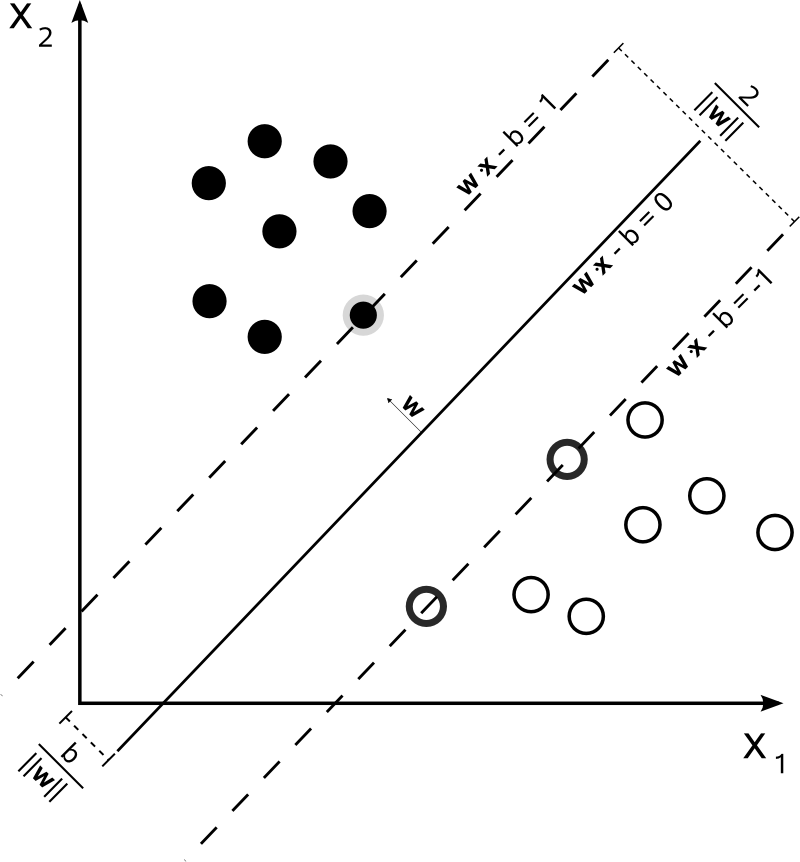
\includegraphics[width=0.5\textwidth, center]{data_classification_svm.png}
			\caption{Support Vector Machine (SVM), an algorithm to classify data}
		\end{figure}
	
	\subsection{Artificial Neural Network}
	In machine learning and cognitive science, artificial neural networks (ANNs) are a family of models inspired by biological neural networks (the central nervous systems of animals, in particular the brain) and are used to estimate or approximate functions that can depend on a large number of inputs and are generally unknown. Artificial neural networks are generally presented as systems of interconnected "neurons" which exchange messages between each other. The connections have numeric weights that can be tuned based on experience, making neural nets adaptive to inputs and capable of learning.

For example, a neural network for handwriting recognition is defined by a set of input neurons which may be activated by the pixels of an input image. After being weighted and transformed by a function (determined by the network's designer), the activations of these neurons are then passed on to other neurons. This process is repeated until finally, an output neuron is activated. This determines which character was read.

Like other machine learning methods – systems that learn from data – neural networks have been used to solve a wide variety of tasks that are hard to solve using ordinary rule-based programming, including computer vision and speech recognition.

A basic model of neural network is displayed in figure \ref{fig:neural_net_model}.

		\begin{figure}[H]
			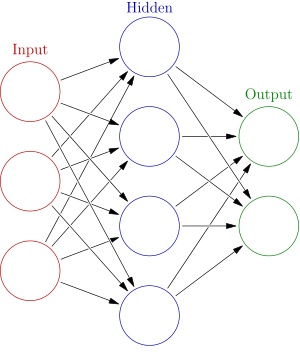
\includegraphics[width=.4\textwidth, center]{neural_net_example.png}
			\caption{Basic model of artificial neural networks}
			\label{fig:neural_net_model}
		\end{figure}
	
	\subsection{Feedforward Neural Network}
	
	A feedforward neural network is an artificial neural network where connections between the units do not form a cycle. This is different from recurrent neural networks.

The feedforward neural network was the first and simplest type of artificial neural network devised. In this network, the information moves in only one direction, forward, from the input nodes, through the hidden nodes (if any) and to the output nodes. There are no cycles or loops in the network.

		\begin{figure}[H]
			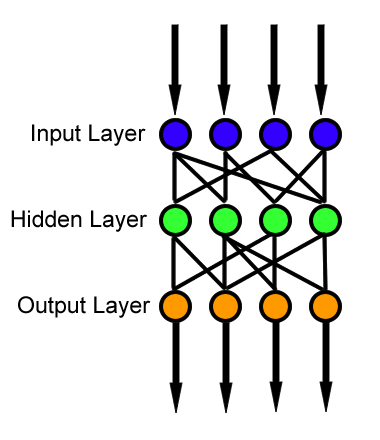
\includegraphics[width=0.4\textwidth, center]{Feed_forward_neural_net.png}
			\caption{A simple Feedforward neural network.}
		\end{figure}
		
		
		\subsubsection{Multi-layer perceptron}
		This class of networks consists of multiple layers of computational units, usually interconnected in a feed-forward way. Each neuron in one layer has directed connections to the neurons of the subsequent layer. In many applications the units of these networks apply a sigmoid function as an activation function.

The universal approximation theorem for neural networks states that every continuous function that maps intervals of real numbers to some output interval of real numbers can be approximated arbitrarily closely by a multi-layer perceptron with just one hidden layer. This result holds for a wide range of activation functions, e.g. for the sigmoidal functions.

		\begin{figure}[H]
			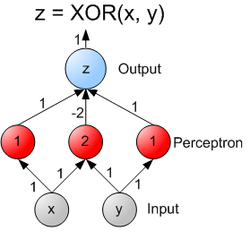
\includegraphics[width=0.4\textwidth, center]{XOR_perceptron_net.png}
			\caption{A multi-layer perceptron network learning XOR}
		\end{figure}
		
		
	\subsubsection{Backpropagation}
	
	Backpropagation, an abbreviation for "backward propagation of errors", is a common method of training artificial neural networks used in conjunction with an optimization method such as gradient descent. The method calculates the gradient of a loss function with respect to all the weights in the network. The gradient is fed to the optimization method which in turn uses it to update the weights, in an attempt to minimize the loss function.
	
	\subsubsection{Gradient descent}
	Gradient descent is a first-order optimization algorithm. To find a local minimum of a function using gradient descent, one takes steps proportional to the negative of the gradient (or of the approximate gradient) of the function at the current point.


	\section{Importance of the project}
	
	Robotics technology is emerging at a rapid pace, offering new possibilities for automating tasks in many challenging applications, especially in autonomous self driving vehicles. A lot of parameters and conditions and other necessary things are needed to be considered to build a complete autonomous self driving vehicles, yet making the vehicle to learn to follow the line of the path is one of the basic building blocks to build a complete autonomous self driving vehicles. The main objective of the project is to train a network and apply it on a autonomous line following prototype which can navigate autonomously at any line consisting of any width.
	


\end{document}